\documentclass{report}

\usepackage[utf8]{inputenc}
\usepackage[backend=biber,sorting=none]{biblatex}
\usepackage[english]{babel}
\renewcommand{\contentsname}{Indice}
\linespread{1.2}

\addbibresource{bibliography.bib}

\usepackage{geometry}
\geometry{a4paper}
\usepackage{graphicx}
\usepackage{float}
\usepackage{hyperref}
\usepackage{csquotes}
\usepackage{caption}
\usepackage{subcaption}

\usepackage{alltt, fancyvrb}
\usepackage{wrapfig}
\usepackage[italian]{cleveref}
\usepackage{mdframed}

\usepackage{longtable}
\usepackage{xr}

\usepackage{color}
\usepackage{xcolor}
\usepackage{listings}
\definecolor{mygray}{rgb}{0.8,0.8,0.8}
\lstset{%
	basicstyle=\ttfamily,
	breaklines = true,
	backgroundcolor=\color{mygray},
}


\definecolor{codegreen}{rgb}{0,0.6,0}
\definecolor{codegray}{rgb}{0.5,0.5,0.5}
\definecolor{codepurple}{rgb}{0.58,0,0.82}
\definecolor{backcolour}{rgb}{0.95,0.95,0.95}
\definecolor{mygray}{rgb}{0.8,0.8,0.8}

\lstdefinestyle{mystyle}{
	backgroundcolor=\color{backcolour},
	commentstyle=\color{codegreen},
	keywordstyle=\color{magenta},
	numberstyle=\tiny\color{codegray},
	stringstyle=\color{codepurple},
	basicstyle=\ttfamily\footnotesize,
	breakatwhitespace=false,
	breaklines=true,
	captionpos=b,
	keepspaces=true,
	numbers=left,
	numbersep=5pt,
	showspaces=false,
	showstringspaces=false,
	showtabs=false,
	tabsize=2
}

\lstset{style=mystyle}

\usepackage{multirow, hhline}
\usepackage{array,booktabs}
\newcolumntype{M}[1]{>{\centering\arraybackslash}m{#1}}

\title{Pervasive Computing project \\ MDM Digital Twins}
\author{Nicolas Farabegoli\\
Linda Vitali}
\date{October 2022}

\begin{document}

\maketitle
\tableofcontents
\clearpage

\chapter{Introduction}
With this project, we have studied, analyzed and provided a prototype solution that models the business processes of \textbf{Caseificio Mambelli} so
that they can benefit from strong technological and digital support going in a direction of integration, resource-saving and innovation.

Following the domain analysis conducted with domain experts, which areas could benefit from Digital Twin support were identified.
As a project challenge, Digital Twin modeling was conducted following some of the Domain Driven Design methodologies.

One of the issues that domain experts have raised is that the information and reports that the machines generate are difficult to find.
Each manufacturer makes its reports or data available through very different formats and applications; all of which make it very difficult
and inconvenient to extrapolate this data and cross-reference it to gain insight into the effectiveness of business processes.
Therefore, through Digital Twin, we want to significantly improve this issue by going in a direction of uniformity of access to machinery
information.
Another aspect that we want to improve is to integrate machinery more closely with the corporate factory system so that they operate in unison.
Finally, we have envisioned how Digital Twins can make machinery smarter by, for example, predicting its breakdowns and preventing failures while
minimizing outages.

All proposed analyses and solutions were made possible through feedback and support from domain experts.
The added value to this project from our point of view is dictated by the fact that it was possible to interact with them and collaborate to find
solutions to concrete problems.

In the intervening period for the development of the project, the company has made adjustments for ``Industria 4.0'' giving us the opportunity to
analyze what requirements are needed and what possible improvements can be applied to move in a direction of innovation.


In the following sections, we will describe the current problems the company is facing and the possible solutions that we have proposed.

\section{Interoperability}
The problem of interoperability in the industrial context has been evident for years now~\cite{LIAO201712434}: each manufacturer produces closed systems, and interoperability with other machines succeeds only if the two parties agree on how to exchange data.
Collaborations between companies often result in tensions and disagreements slowing system development and generating a sub-optimal quality product.
In addition, such collaborations are created ad-hoc, so the methodologies and tools used can vary significantly going to making further integration
with other systems or devices difficult if not impossible.

In the manufacturing domain, interoperability represents a characteristic of a manufacturing system in which its components are capable of exchanging information with one another, using the information that has been exchanged.
Studies have been conducted on how interoperability is viewed at the industrial level. One study found that the automotive industry is strongly interested in achieving a high degree of interoperability, whereas the food industry perceives almost no need to have interoperable systems between them~\cite{LIAO201712434}. Only the 16\% of the food industry is interested in achieving a high degree of interoperability, compared with the 60\% of the automotive industry (Figure~\ref{fig:interoperability}).

\begin{figure}[h]
	\centering
	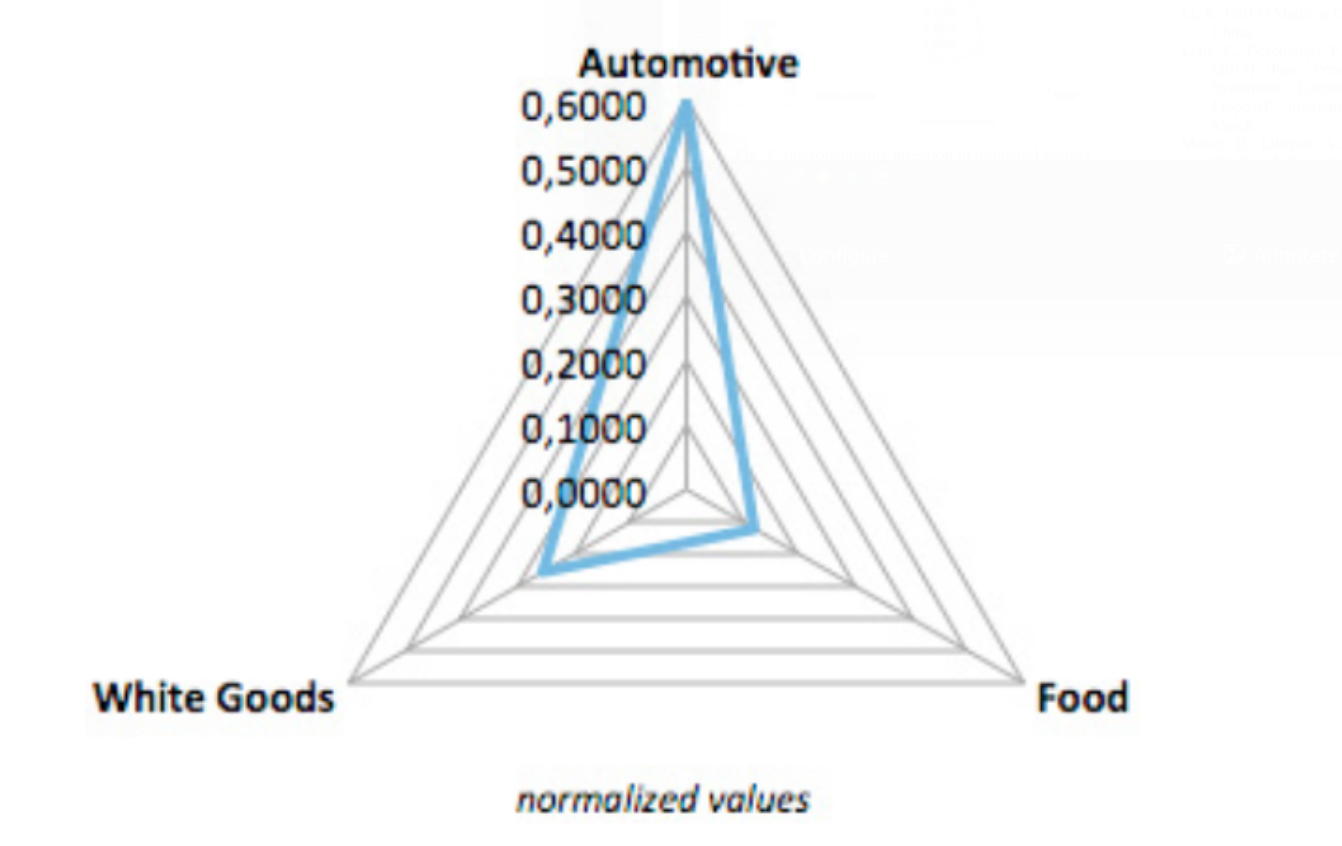
\includegraphics[width=0.6\textwidth]{img/interoperability.png}
	\caption{Interoperability attention in industrial sectors}
	\label{fig:interoperability}
\end{figure}

The results provided by the study are corroborated by the fact that domain experts initially did not perceive interoperability as beneficial, but
with the advent of \textit{Industry 4.0}, they have realized how interoperability is critical to the proper functioning of the system.

Currently, aspects of interoperability between machines are not present in the company.
Each machine in the production and packaging line is manually configured by an operator.
As can be easily guessed, this kind of operation can be error-prone, so having interoperability between machines that enable the communication of
information needed for that specific processing turns out to be a fundamental requirement in \textit{Industry 4.0}

Over time, several frameworks and standards have been proposed that aim to achieve a high degree of interoperability in the Industrial Internat of
Things. Among the most promising and interesting is the W3C Web of Things specification.
This specification keeps the promise to counter the fragmentation of the Internet of Things by defining a Web-based abstraction layer for existing
platforms, devices, gateways and services.
By complementing existing standards, it enhances interoperability thereby reducing the risk for investors and customers.
This will also enable the rapid growth of open markets for devices and services.

\begin{figure}[h]
	\centering
	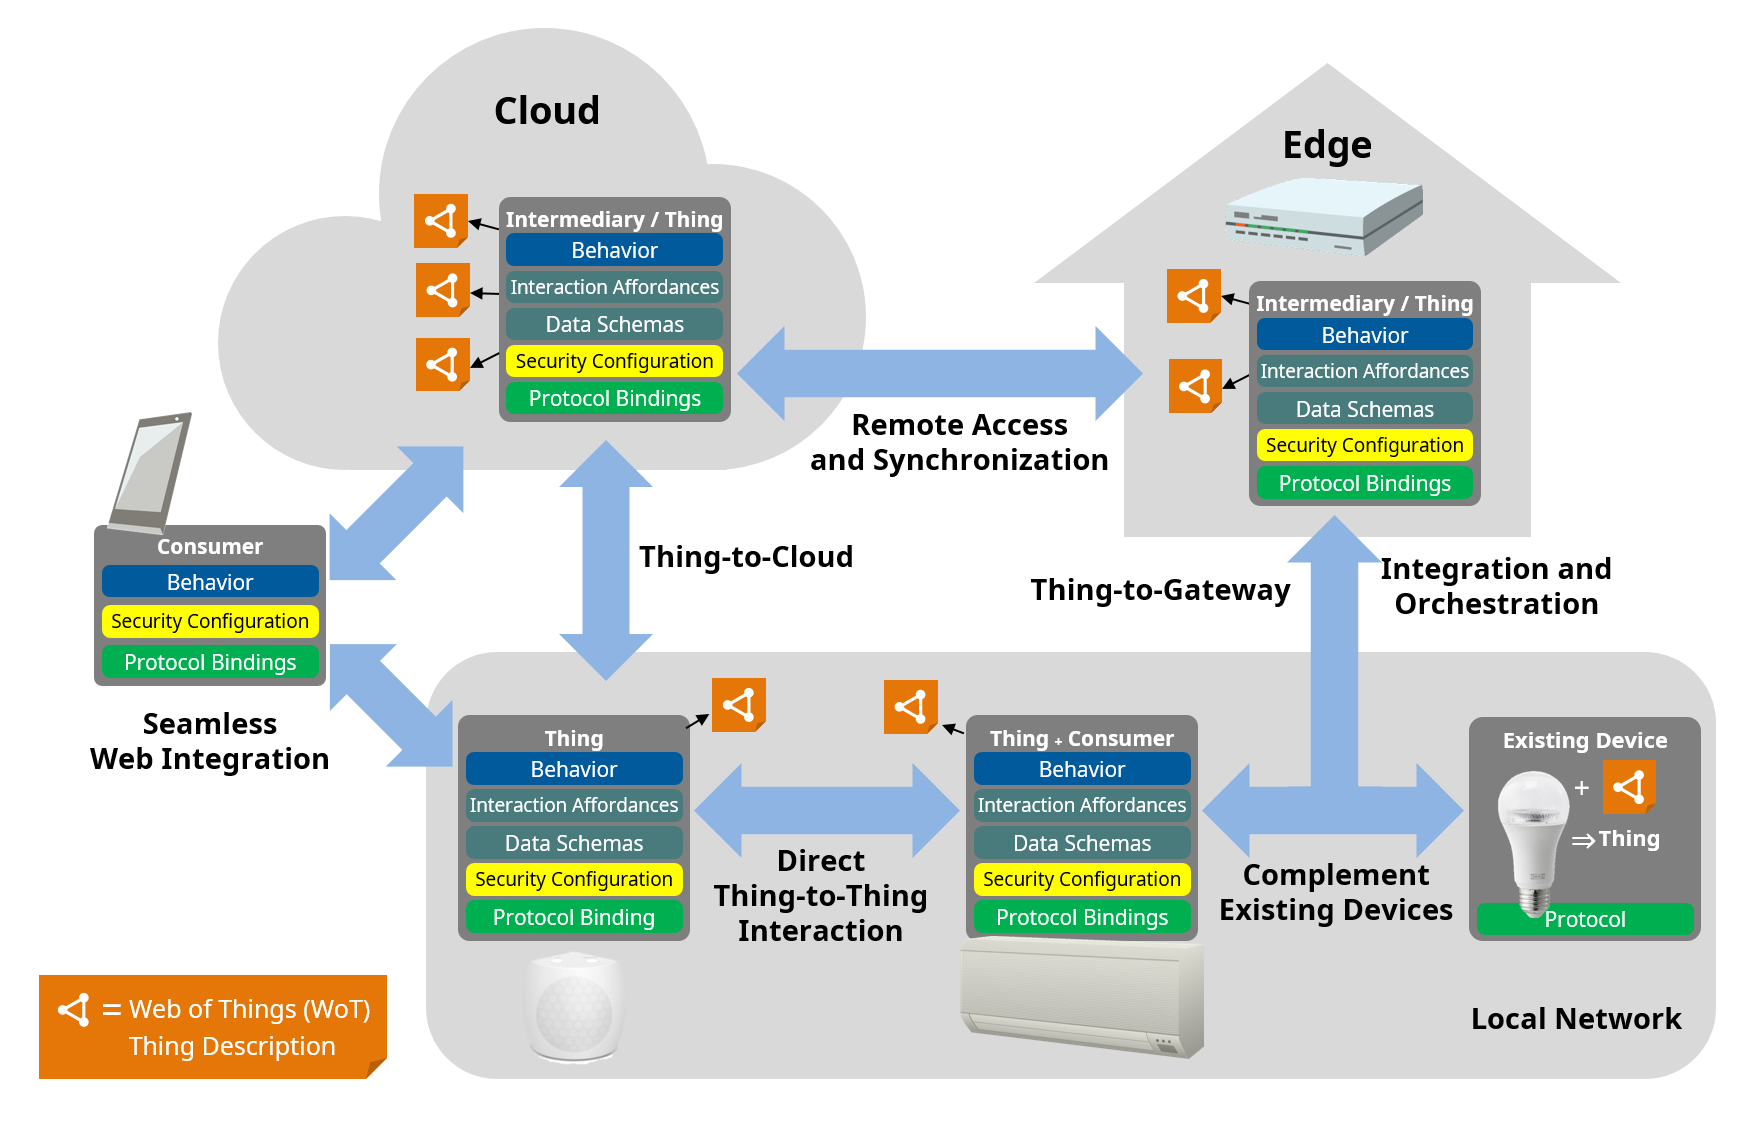
\includegraphics[width=0.7\textwidth]{img/wot.png}
	\caption{Web of Things architecture}
	\label{fig:iot}
\end{figure}

The Web of Things architecture (Figure~\ref{fig:iot}) shows how the interoperability between devices and systems is the main aspect.
In our opinion, the WoT specification is one of the most promising and interesting specifications for the development of interoperable systems.
Moreover, this specification joint with the Digital Twin pattern could represent a fundamental step towards interconnected digital systems.

\section{Industria 4.0}
Industry 4.0 is the propensity of today's industrial automation to incorporate some new production technologies to improve working conditions, create
new business models, increase plant productivity and improve product quality.
In developing this project, we took into consideration the goals of \textit{Industry 4.0}. Although it represents a way to obtain funding,
in this project, we analyzed the technical part and observed what improvements it aspires and what the current limitations are.


One of the most relevant aspects is that it is required that machinery in \textit{Industry 4.0} be interconnected with the factory information
system. It is also required that the information that these machines generate, must be integrated with the company's data.
Another required feature is remote control of machine settings, thus avoiding the need for the operator to set the machine.

As can be observed, the standard provides for strong interconnection of machinery and attaches great value to the data provided to such an extent that it forces the integration of these data with those already present. It also places a strong emphasis on automation, delegating configuration operations to the information system as much as possible, and limiting human intervention to only rare and exceptional cases.

\chapter{Architecture}
The architecture of each bounded context follows the Clean Architecture's structure: Entities, Use Cases, Interface Adapters, Frameworks and Drivers.

\begin{itemize}
    \item The first layer consists of the domain Aggregates we named Types; these are the domain entities and are the least likely to change when something external changes
    \item The second layer is composed of the domain ``Actions'', namely the business processes to model and ``Domain Events'': the starting point for almost all the business processes. They orchestrate the flow of data to and from the entities of the layer below
    \item For the Interface Adapters layer, in order to protect the layers underneath, we built Data Transfer Objects (DTOs) for every element that has to be transferred towards other bounded contexts or be persisted in storage. We also used the Repository pattern to abstract over the particular data persistence infrastructure. DTOs were also used in the Anti-Corruption Layer and Open-Host Service patterns to convert and present external data to the Entities and Use Case layers
    \item As for the Frameworks and Drivers layer, it contains the minimal amount of code needed to glue together the ``communication code'' (HTTP servers, Database persistence, etc.) with the code below. We implemented the HTTP servers belonging to this layer and mocked the remaining code related to data persistence or message-oriented communication.
    
    However, we did not mock the code necessary to communicate with the digital twins.
    We allowed the transfer of information with the usage of WebSockets, so we could receive data and events sent directly from the digital twins.
\end{itemize}


\begin{figure}[H]
    \centering
    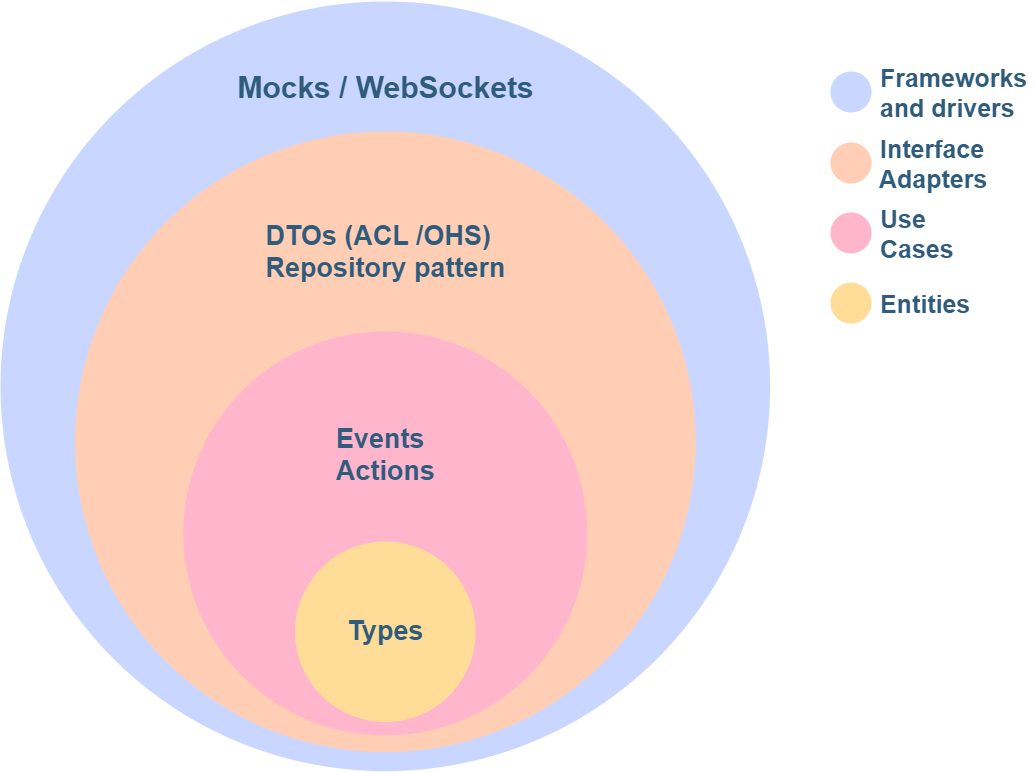
\includegraphics[width=0.8\textwidth]{img/clean-architecture.png}
    \caption{Bounded Contexts architecture}
    \label{img:clean-architecture}
\end{figure}

\section{Context Map}
In this chapter, we analyzed the bounded contexts related to digital twins and their relationships.
The context map in figure \ref{img:context-map} represents the relationships patterns between the bounded contexts.

\begin{itemize}
    \item \textbf{MilkPlanning [D, ACL] $\leftarrow$ [U] MilkTankDT}
    
    \texttt{MilkPlanning} receives the information about the tanks' milk quantity from the \texttt{MilkTankDT}.
    \texttt{MilkPlanning} is a downstream bounded context and has an Anti-Corruption Layer.
    
    \item \textbf{Stocking [D, ACL] $\leftarrow$ [U] PackagingMachineDT \\ 
    Stocking [D, ACL] $\leftarrow$ [U] ScaleDT \\ 
    Stocking [D, ACL] $\leftarrow$ [U] MetalDetectorDT}

    \texttt{Stocking} receives the information about the quality assurance status considering the packaging machine, scale and metal detector. Data are sent from the \texttt{PackagingMachineDT}, \texttt{ScaleDT} and \texttt{MetalDetectorDT} respectively.
    \texttt{Stocking} is a downstream bounded context and has an Anti-Corruption Layer.
	
	\item \textbf{Alert [D, ACL] $\leftarrow$ [U] MilkTankDT \\
	Alert [D, ACL] $\leftarrow$ [U] MetalDetectorDT \\
	Alert [D, ACL] $\leftarrow$ [U]PackagingMachineDT \\
	Alert [D, ACL] $\leftarrow$ [U]ScaleDT}

    \texttt{Alert} receives the alerting messages from the digital twins. Data are sent from the \texttt{MilkTankDT}, \texttt{MetalDetectorDT}, \texttt{PackagingMachineDT} and \texttt{ScaleDT} respectively.
    \texttt{Alert} is a downstream bounded context and has an Anti-Corruption Layer.

    \item \textbf{MilkPlanning [D, ACL] $\leftarrow$  [U] Stocking} 
    
    \texttt{MilkPlanning} asks \texttt{Stocking} for the amount of products in stock.
    \texttt{MilkPlanning} is a downstream bounded context and has an Anti-Corruption Layer.

    \item \textbf{Alert[D, ACL] $\leftarrow$  [U] Maintenance}
    
    \texttt{Maintenance} sends the alerting messages about machine failure to \texttt{Alert}.
    \texttt{Alert} is a downstream bounded context and has an Anti-Corruption Layer.

	\item \textbf{Maintenance[D, ACL] $\leftarrow$  [U] PackagingMachineDT}
	
    \texttt{Maintenance} receives the information about the packaging machine status from \texttt{PackagingMachineDT} in order to forecast packaging machine failures.
    \texttt{Maintenance} is a downstream bounded context and has an Anti-Corruption Layer.

	\item \textbf{Reporting[D] $\leftarrow$  [U] ScaleDT \\
    Reporting[D] $\leftarrow$  [U] MetalDetectorDT }

    \texttt{Reporting} receives information from \texttt{ScaleDT} and \texttt{MetalDetectorDT} about their status in order to generate reports.
	

\end{itemize}

\begin{figure}[H]
    \centering
    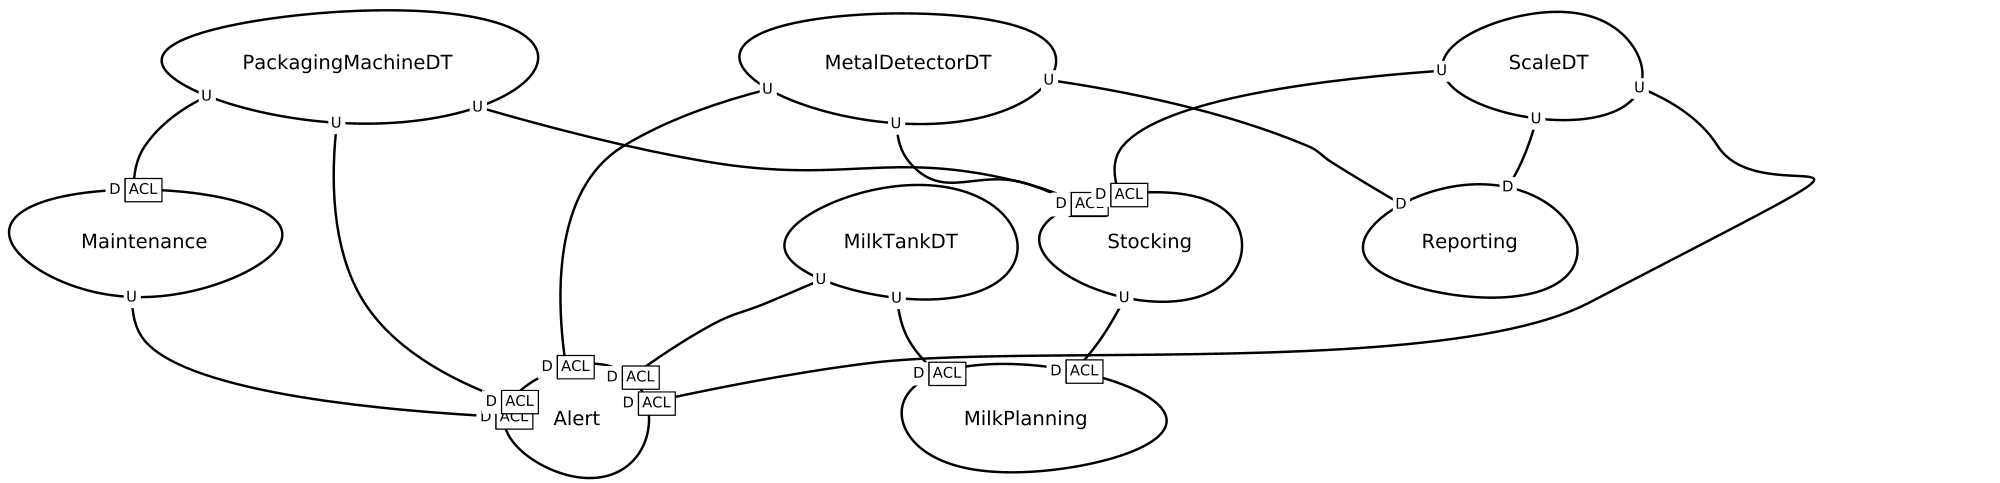
\includegraphics[width=\textwidth]{img/context-map.png}
    \caption{Context Map}
    \label{img:context-map}
\end{figure}



\chapter{Digital Twins description}

\section{Digital twins for machines}
\subsection{Milk Tank}
\subsubsection{Thing Model}
Properties: Manufacturer, Serial number, pH, minPH, maxPH, temperature, minTemp, maxTemp, quantityOfmilk
Events: temperatureOutOfRange, pHoutOfRange
Actions: Open Valve

\section{Digital twins for anticipazione guasti}
\subsection{Packaging machine}
\subsubsection{Thing Model}
Properties: Manufacturer, Serial number, currentBatch, cutterTemperature
Events: packagingStarted, packagingMachineFailure, packageDamaged,
<<<<<<< HEAD
Action: startPackaging

% cutterTemperature viene passato all'algoritmo che in caso di packagingMachineFailure o packageDamaged poi vede che magari la temperatura era troppo alta e capisce qual era il problema
=======
Action: Start Packaging
>>>>>>> 69156db... chore: useful comments

% cutterTemperature viene passato all'algoritmo che in caso di packagingMachineFailure o packageDamaged poi vede che magari la temperatura era troppo alta e capisce qual era il problema

riceve le info su quale lotto deve iniziare a confezionare così da impostare automaticamente i parametri della macchina.
tramite algoritmo di machine learning, la macchina predice il guasto e lo comunica tramite alert.
I parametri che valuta sono: numero di chiusure al minuto per tipo di prodotto, numero di confezioni danneggiate, temperatura resistenza saldatore (cutter).

\section{Digital twins for quality assurance}
DT a livello di processo. Quello per la QA(metal detector e scale) viene creato e distrutto all'interno di un ciclo di valutazione di un lotto.
Si collega ai DT del metal detector e della bilancia per effettuare la QA.
\subsection{Metal detector}
\subsubsection{Thing Model}
Properties: Manufacturer, Serial number, currentBatch
Events: numberOfDroppedPackages

Rifiuta il batch se almeno un prodotto viene rilevato come non conforme, altrimenti invia il batch al successivo step.
I parametri sono:
numero di prodotti rilevati come non conformi appartenenti ad un determinato lotto

\subsection{Scale}

\subsubsection{Thing Model}
Properties: Manufacturer, Serial number, currentBatch, meanWeight, stdDevWeight
Events: numberOfDroppedPackages, batchCompleted

Approva in automatico il batch se tutti i prodotti vanno bene, altrimenti rifiuta tutto il batch obbligando l'operatore ad intervenire manualmente.
I parametri sono:
per ogni lotto il numero di confezioni pesate, il numero di confezioni che superano il peso minimo e il numero di confezioni che superano il peso massimo, il peso medio per lotto, la deviazione standard per lotto

\chapter{Bounded Contexts}
\section{Milk Planning}
% incollare parte del bc del Milk Planning
\section{Milk Tank}
% storiella di cosa è il milk tank

\section{More bounded contexts}
Other bounded contexts that are not part of the scope of this project can be found here: \url{https://atedeg.dev/mdm/_docs/index.html}
\chapter{Context Map}
In this chapter, we analyzed the bounded contexts related to digital twins and their relationships.
The context map in figure \ref{img:context-map} represents the relationships patterns between the bounded contexts.

\begin{itemize}
    \item \textbf{MilkPlanning [D, ACL] $\leftarrow$ [U] MilkTankDT}
    
    \texttt{MilkPlanning} receives the information about the tanks' milk quantity from the \texttt{MilkTankDT}.
    \texttt{MilkPlanning} is a downstream bounded context and has an Anti-Corruption Layer.
    
    \item \textbf{Stocking [D, ACL] $\leftarrow$ [U] PackagingMachineDT \\ 
    Stocking [D, ACL] $\leftarrow$ [U] ScaleDT \\ 
    Stocking [D, ACL] $\leftarrow$ [U] MetalDetectorDT}

    \texttt{Stocking} receives the information about the quality assurance status considering the packaging machine, scale and metal detector. Data are sent from the \texttt{PackagingMachineDT}, \texttt{ScaleDT} and \texttt{MetalDetectorDT} respectively.
    \texttt{Stocking} is a downstream bounded context and has an Anti-Corruption Layer.
	
	\item \textbf{Alert [D, ACL] $\leftarrow$ [U] MilkTankDT \\
	Alert [D, ACL] $\leftarrow$ [U] MetalDetectorDT \\
	Alert [D, ACL] $\leftarrow$ PackagingMachineDT \\
	Alert [D, ACL] $\leftarrow$ ScaleDT}

    \texttt{Alert} receives the alerting messages from the digital twins. Data are sent from the \texttt{MilkTankDT}, \texttt{MetalDetectorDT}, \texttt{PackagingMachineDT} and \texttt{ScaleDT} respectively.
    \texttt{Alert} is a downstream bounded context and has an Anti-Corruption Layer.

    \item \textbf{MilkPlanning [D, ACL] $\leftarrow$  [U] Stocking} 
    
    \texttt{MilkPlanning} asks \texttt{Stocking} for the amount of products in stock.
    \texttt{MilkPlanning} is a downstream bounded context and has an Anti-Corruption Layer.

\end{itemize}

\begin{figure}[H]
    \centering
    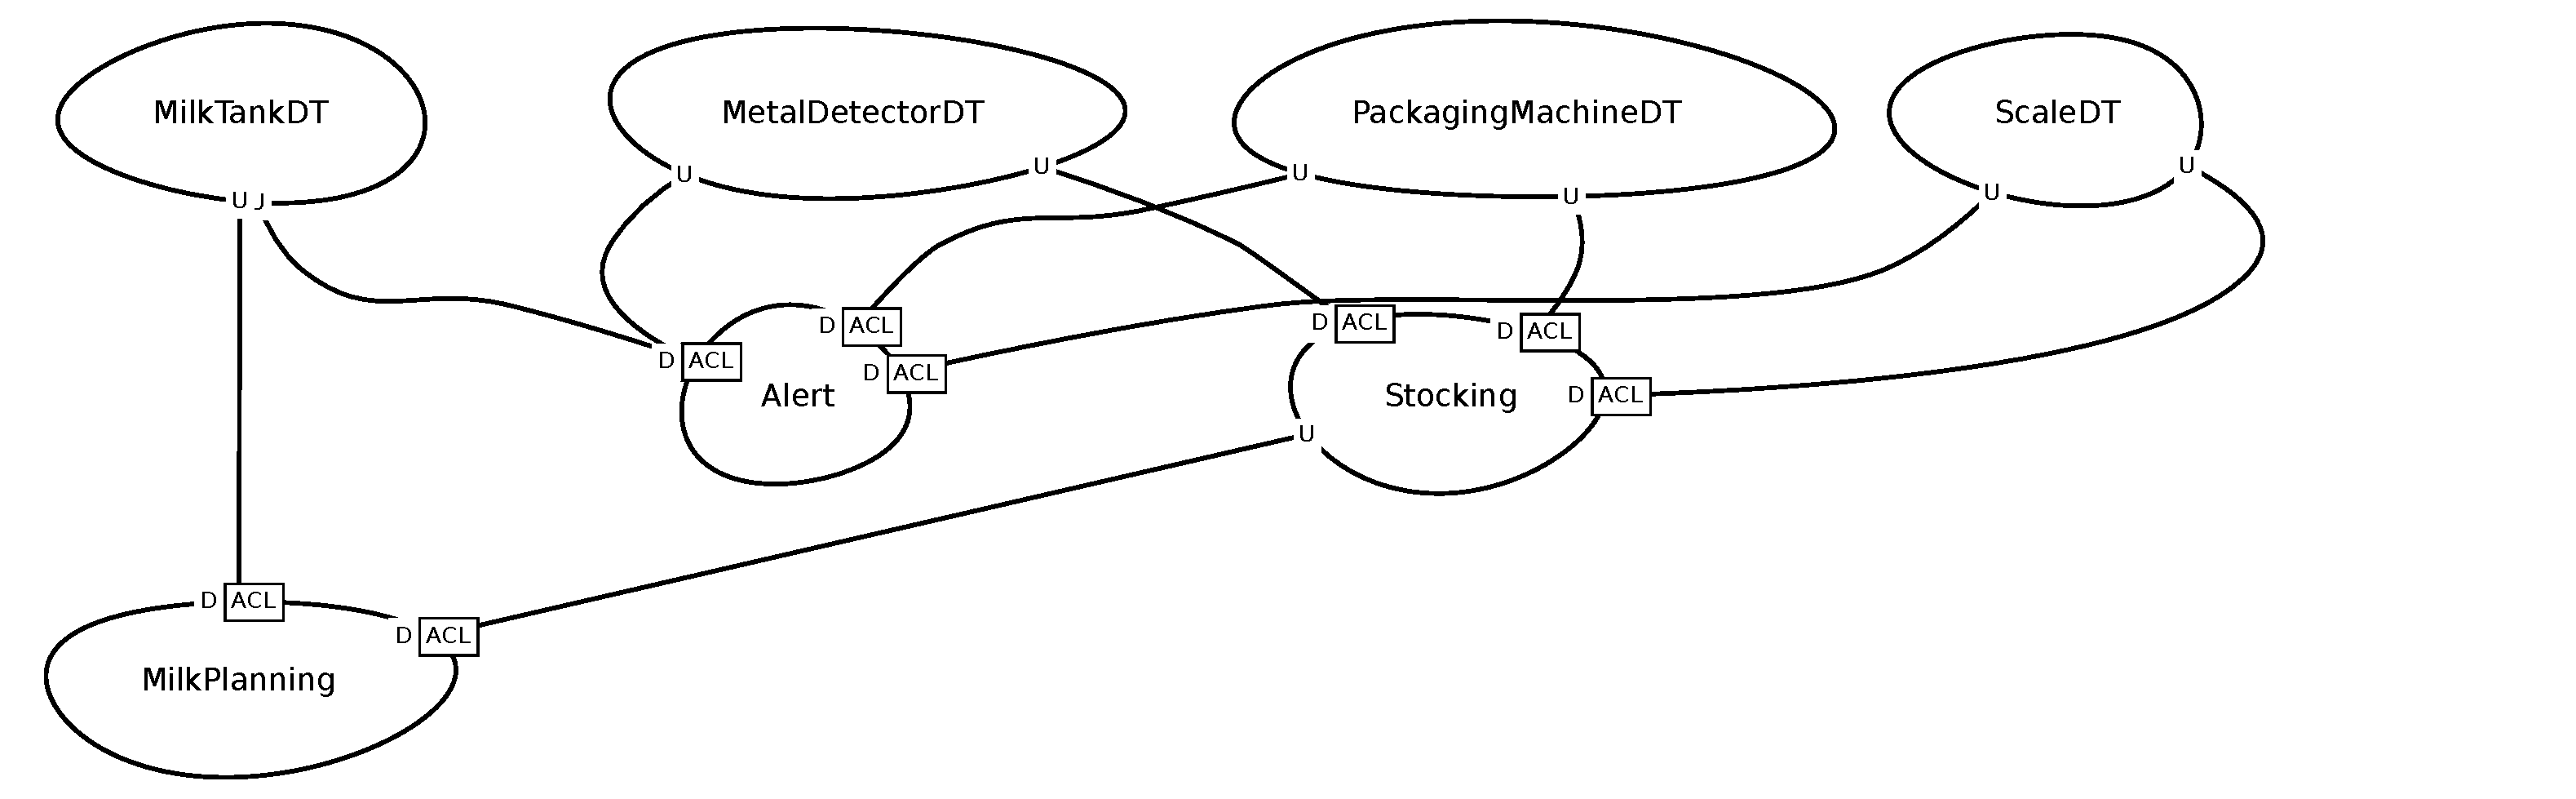
\includegraphics[width=\textwidth]{img/contextMap.eps}
    \caption{Context Map}
    \label{img:context-map}
\end{figure}




\end{document}
